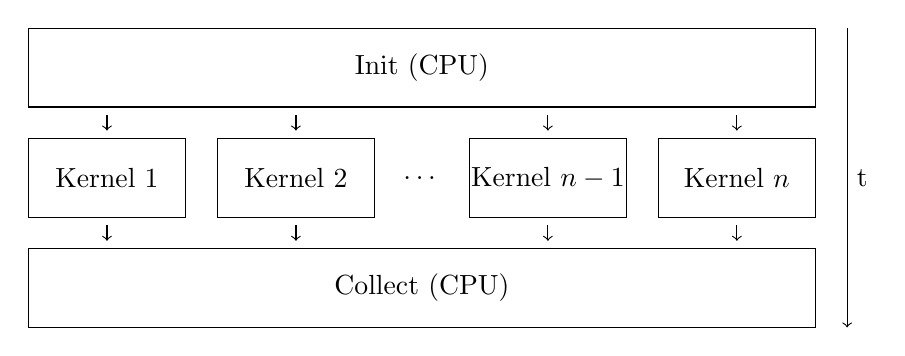
\begin{tikzpicture}

	% Init
	\draw (0,2.8) rectangle node {Init (CPU)} (10,3.8);

	% Kernels
	\draw (0,1.4) rectangle node {Kernel $1$} (2,2.4);
	\draw (2.4,1.4) rectangle node {Kernel $2$} (4.4,2.4);
	\draw (5,1.9) node {\ldots};
	\draw (5.6,1.4) rectangle node {Kernel $n-1$} (7.6,2.4);
	\draw (8,1.4) rectangle node {Kernel $n$} (10,2.4);

	% Collect
	\draw (0,0) rectangle node {Collect (CPU)} (10,1);

	% Time arrow
	\draw[<-] (10.4,0) -- node [right] {t} (10.4,3.8);

	% Flow arrows
	\foreach \x in {1, 3.4, 6.6, 9} {
		\draw[<-] (\x,1.1) -- (\x,1.3);
		\draw[<-] (\x,2.5) -- (\x,2.7);
	}

\end{tikzpicture}
